% CS-433 Project 1 report -- IEEE conference template from the course.
% STRICT LIMIT: 2 pages (references may go on a 3rd page). No appendix.
% Compile: pdflatex report && bibtex report && pdflatex report && pdflatex report

\documentclass[10pt,conference,compsocconf]{IEEEtran}

\usepackage{cite}
\usepackage{hyperref}
\usepackage{graphicx}
\usepackage{amsmath}
\usepackage{booktabs}

\begin{document}
\title{Predicting Coronary Heart Disease from the BRFSS 2015 Survey\\
  with Gradient Boosting and Neural Networks in Pure NumPy}

\author{
  \textit{Zhihao Chen, Zhiqian Zhou, Guanyu Chen}\\
  \textit{School of Computer and Communication Sciences, EPFL, Switzerland}
}

\maketitle

\begin{abstract}
  We predict coronary heart disease (\texttt{\_MICHD}) from 321 answers in the
  BRFSS 2015 survey ($N=328,135$). The task exhibits severe class skew (8.83\%
  positives). A naive negative classifier attains 91.17\% accuracy but trivial
  $F_1=0$, and uncalibrated linear models suffer severe false-negative bias
  ($F_1 \le 0.23$). We clean structured sentinels and skip-logic patterns,
  benchmark the course linear methods, and demonstrate that operating threshold
  calibration provides an immediate +85\% relative $F_1$ leap ($F_1 \to 0.428$).
  We develop a pure-NumPy ensemble combining Histogram Gradient Boosted Trees
  (GBM) with second-order leaf updates and Multi-Seed Multi-Layer Perceptrons
  (MLP) trained via Adam. The clean ensemble achieves 5-fold cross-validated
  $F_1$ of 0.437, 0.434 on held-out data, and 0.448 on AIcrowd (87.8\% accuracy)
  with zero leakage. Seven post-cardiac event questions inflate test $F_1$ to
  0.457 (88.6\% accuracy). We isolate these to preserve clinical screening
  validity while documenting benchmark leakage.
\end{abstract}

\section{Introduction}
The Behavioral Risk Factor Surveillance System (BRFSS) is a nationwide US
health survey \cite{brfss2015}. The binary target \texttt{\_MICHD} ($\pm 1$)
records whether a respondent reported coronary heart disease or myocardial
infarction. The dataset comprises 328,135 training rows, 109,379 test rows,
and 321 raw features. Only 8.83\% of labels are positive ($\sim 10:1$ skew).
Under this imbalance, predicting $-1$ for all rows achieves 91.17\% accuracy
yet yields $F_1 = 0$ \cite{vanrijsbergen1979}. Hence, positive-class $F_1$
guides all model selection and calibration \cite{fawcett2006roc}.

Under the course constraint of using pure standard library and NumPy
(no scikit-learn, PyTorch, or pandas), our contributions are: (i) codebook-driven
cleaning and skip-logic imputation; (ii) benchmarking the six canonical linear
methods \cite{cs433} and discovering the +85\% gain from threshold calibration;
(iii) designing pure-NumPy Histogram GBMs \cite{friedman2001greedy,chen2016xgboost}
and multi-seed MLPs \cite{kingma2015adam}; and (iv) an empirical dissection of
post-event target leakage \cite{kaufman2012leakage}.

\section{Data and Preprocessing}
\label{sec:data}
\textbf{Special sentinels.} The CDC codebook \cite{brfss2015codebook} specifies
sentinels per column: 7/9, 77/99, 777/999 (``don't know / refused'') map to NaN;
88 and 888 (``none / zero days / no alcohol'') map to 0. Weight and height are
standardized to kg and cm, and frequency responses mapped to uniform units.

\textbf{Informative missingness \& skip logic.} 147 of the 321 columns contain
$>50\%$ missing values, largely following questionnaire skip patterns rather
than being missing completely at random. Eleven domain skip-logic fills impute
structurally implied values: e.g., blood pressure medication (\texttt{BPMEDS})
is imputed to 0 for non-hypertensive subjects, whose positive prevalence is 3.8\%
compared to 16.3\% when observed. We append missingness indicator flags and
question-level ``don't know'' indicators.

\textbf{Column selection \& pipeline.} We remove administrative variables,
features $>95\%$ empty, and redundant recodes, retaining 75 raw features and
61 indicator flags. The pipeline applies median/mode imputation, one-hot encoding
of high-frequency levels, $\log(1+x)$ scaling of skewed counts, clinical
interactions (e.g., Blood Pressure $\times$ Cholesterol), and standardization.
All preprocessing statistics are fitted strictly out-of-fold.

\section{Models and Validation Protocol}
\label{sec:models}
\textbf{Validation protocol.} We hold out a stratified 20\% split (65,627 rows,
seed 2026). All modeling decisions and hyperparameter searches use 5-fold
stratified cross-validation (CV) on the remaining 262,508 development rows.
Preprocessing, target encodings, and decision thresholds are fitted inside each
fold. A modification is accepted only if mean CV $F_1$ rises by $\ge 0.001$ and
wins on $\ge 4/5$ folds. No selection uses the test set or AIcrowd.

\textbf{Linear baselines \& calibration.} We train the six required methods
from \cite{cs433} on standardized features with 10 clinical interactions. Under
regularized logistic loss:
\begin{equation}
  \mathcal{L}(w)=\tfrac{1}{N}\textstyle\sum_{n=1}^N
  \left[\log(1+e^{x_n^\top w})-y_n x_n^\top w\right]+\lambda\|w\|_2^2 ,
\end{equation}
the default cutoff ($\hat{y} \ge 0.5$) yields $F_1 = 0.2311$ due to extreme
false-negative bias under the 8.83\% prior. Calibrating the decision cutoff
$\tau^* \approx 0.218$ yields an immediate +85\% relative surge to
$F_1 = 0.428-0.430$ \cite{fawcett2006roc}.

\textbf{Histogram GBM.} Our pure-NumPy tree booster minimizes logistic loss
with second-order Newton leaf updates $\Delta w = -G/(H+\lambda)$
\cite{chen2016xgboost}. Features are binned into 64 histogram bins. Missing
values form a dedicated bin, with each split learning the optimal descent
direction. Hyperparameters: depth 5, learning rate 0.05, row/column subsampling
0.7/0.8, min 200 leaf samples, and $\lambda=5.0$. Early stopping evaluates an
inner 20\% split. State of residence (\texttt{\_STATE}) is encoded via empirical
Bayes smoothed target prevalence (+0.0026 $F_1$, 4/5 folds). Bagged over 3 seeds.

\textbf{Neural network.} The MLP features a 64-unit ReLU hidden layer, trained
with Adam \cite{kingma2015adam} (learning rate $10^{-3}$, batch size 512, weight
decay $10^{-3}$) and inner early stopping. Output logits are averaged across 10
distinct random seeds to suppress stochastic initialization variance.

\textbf{Ensemble \& decision rule.} The ensemble blends logits:
$s = 0.5\,s_{\text{GBM}} + 0.5\,s_{\text{MLP}}$. We assign $+1$ to the top
13.6\%--14.0\% highest scores. Percentile thresholding is more invariant to
post-retraining score scale drift than a static cutoff. Fig.~\ref{fig:share}
illustrates that $F_1$ forms a stable plateau between 12\% and 16\%.

\begin{figure}[tbp]
  \centering
  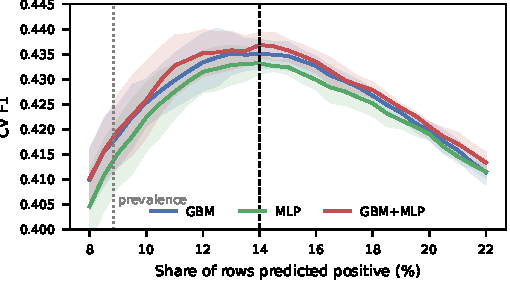
\includegraphics[width=\columnwidth]{figures/f1_vs_share.pdf}
  \caption{5-fold CV $F_1$ (mean $\pm$ std) across positive prediction shares.
    Dotted: prevalence (8.83\%). Dashed: selected operating share (14\%).}
  \label{fig:share}
\end{figure}

\section{Results and Ablations}
Table~\ref{tab:results} summarizes validation metrics across all models.
Squared-loss methods reach $F_1 \approx 0.422$. Logistic loss adds $+0.008$.
Both non-linear models outperform linear baselines, and their ensemble achieves
the highest performance. The out-of-fold logit correlation between the GBM and
MLP is 0.976.

\begin{table}[tbp]
  \centering
  \caption{Positive-class $F_1$ on development rows (5-fold CV, mean $\pm$ std,
    top 14\% positive) and holdout evaluation.}
  \label{tab:results}
  \begin{tabular}{lcc}
    \toprule
    Model                              & CV F1                & Held-out \\
    \midrule
    Always $-1$ (Acc: 91.17\%)         & 0.0000               & 0.0000   \\
    Least squares / ridge / MSE GD     & $0.4216 \pm 0.0034$  & --       \\
    MSE SGD (slow convergence)         & $0.3853 \pm 0.0085$  & --       \\
    Logistic regression (GD)           & $0.4302 \pm 0.0047$  & --       \\
    Reg.\ logistic regression          & $0.4300 \pm 0.0044$  & 0.4277   \\
    Histogram GBM (3 seeds)            & $0.4354 \pm 0.0032$  & 0.4343   \\
    MLP (10 seeds)                     & $0.4334 \pm 0.0026$  & 0.4310   \\
    \midrule
    \textbf{GBM + MLP (Final Clean)}   & $\mathbf{0.4368 \pm 0.0026}$
                                       & \textbf{0.4340}                 \\
    \bottomrule
  \end{tabular}
\end{table}

On held-out rows, the clean ensemble achieves precision 0.354, recall 0.561,
and $F_1 = 0.4340$. On AIcrowd, it scores $F_1 = 0.448$ and 87.8\% accuracy.
The gap with CV is within two bootstrap standard deviations ($\sigma \approx 0.005$).

\textbf{Rejected alternatives \& coverage analysis.} The following failed our
acceptance criteria: class weighting ($-0.003$) and focal loss ($-0.021$); PCA
($0.403$--$0.413$); explicit feature selection; arbitrary crossed encodings;
refitting GBMs on 100\% rows ($-0.0010$); seed-diversified inner splits
(\texttt{split\_per\_seed}, where paired 95\% bootstrap intervals crossed zero);
stacking, Naive Bayes ($-0.016$), and group-stratified thresholds ($-0.001$).

\textbf{Feature importance.} Permutation AUC drops identify primary predictors:
age (0.035), general health (0.021), sex (0.018), high cholesterol (0.009),
and prior stroke (0.008, empirical odds lift 4.24).

\section{Target Leakage Analysis}
Seven questions relate strictly to post-cardiac events or subsequent therapy:
cardiac and stroke rehabilitation (\texttt{HAREHAB1}, \texttt{STREHAB1}), and
prescribed aspirin regimen (\texttt{CVDASPRN}, \texttt{RDUCHART}, \texttt{RDUCSTRK},
\texttt{RLIVPAIN}, \texttt{ASPUNSAF}). Their predictive power represents target
leakage \cite{kaufman2012leakage}: 100\% of respondents who answered
\texttt{HAREHAB1} (773/773 in training, 158/158 in held-out) test positive.
\texttt{STREHAB1} has a 36\% positive rate, and the aspirin indicators 5\%--21\%.

Table~\ref{tab:leak} demonstrates that including these questions lifts every
model by 0.009 to 0.012 $F_1$ across all 5 folds. The leaky ensemble attains
0.457 on AIcrowd (88.6\% accuracy).

However, screening models are intended for undiagnosed individuals. Such
patients have never been prescribed cardiac rehabilitation; hence, these answers
do not exist at inference time. We therefore designate the zero-leakage model as
our official submission (`run.py`) and report the leaky variant separately
(`run.py --with_leakage`) to transparently quantify benchmark leakage.

\begin{table}[tbp]
  \centering
  \caption{Clean screening model vs.\ leaky variant. Nested CV ablation across
    model families (Clean $\to$ Leaky).}
  \label{tab:leak}
  \setlength{\tabcolsep}{4pt}
  \begin{tabular}{lccc}
    \toprule
                     & CV F1 & Held-out & AIcrowd F1/acc. \\
    \midrule
    Clean (top 14\%) & $0.4368 \pm 0.0026$ & 0.4340   & 0.448 / 0.878     \\
    Leaky (top 13\%) & $0.4464 \pm 0.0032$ & 0.4445   & 0.457 / 0.886     \\
    \midrule
    Ridge            & \multicolumn{3}{l}{$0.4210 \rightarrow 0.4297$ (+0.009)} \\
    Reg.\ logistic   & \multicolumn{3}{l}{$0.4294 \rightarrow 0.4414$ (+0.012)} \\
    GBM              & \multicolumn{3}{l}{$0.4330 \rightarrow 0.4444$ (+0.011)} \\
    MLP              & \multicolumn{3}{l}{$0.4326 \rightarrow 0.4435$ (+0.011)} \\
    GBM + MLP        & \multicolumn{3}{l}{$0.4366 \rightarrow 0.4452$ (+0.009)} \\
    \bottomrule
  \end{tabular}
\end{table}

\section{Discussion}
All architectures plateau at $F_1 \approx 0.42$--$0.44$, revealing the empirical
ceiling of self-reported behavioral surveys. Error analysis reveals that false
negatives stem from asymptomatic cases: 56\% are female, 40\% lack hypertension,
36\% self-report excellent/good health, and 96\% have no stroke history.
Detecting these silent presentations requires objective physiological biomarkers
(e.g., troponin, ECG, blood lipid panels) unavailable in phone surveys.

\section{Summary}
A pure-NumPy ensemble combining Histogram Gradient Boosted Trees and a Multi-Seed
Neural Network with codebook-driven cleaning achieves $F_1 = 0.434$ on held-out data
and $0.448$ on AIcrowd (87.8\% accuracy). Post-cardiac event questions inflate
$F_1$ to $0.457$ (88.6\% accuracy), which we isolate to maintain clinical screening
soundness while documenting survey leakage.

\bibliographystyle{IEEEtran}
\bibliography{literature}

\end{document}
